\section{Wielomian Interpolacyjny Lagrange'a}

\begin{frame}{3.5 Wielomian Interpolacyjny Lagrange'a \\ 3.5.1 Interpolacja liniowa}


$P_{1}(x)$ -- przez $(x_{0},\ y_{0})$ i $(x_{1},\ y_{1})$
$$
P_{1}(x)=\underbrace{\frac{(x-x_{1})}{(x_{0}-x_{1})}}_{L_0(x)}y_{0}+\underbrace{\frac{(x-x_{0})}{(x_{1}-x_{0})}}_{L_1(x)}y_{1}=\sum_{k=0}^{1}L_{k}(x)f(x_{k})
$$
\begin{itemize}
\item wielomian stopnia $\leq 1$

\item $x=x_{0}\rightarrow P(x_{0})=y_{0}$ \\
$x=x_{1}\rightarrow P(x_{1})=y_{1}$ \\
$L_{k}(x_{l})=\delta_{k,l}$ \\
\end{itemize}
\begin{flushright}Czy jest jedynym takim wielomianem?\end{flushright}

\end{frame}


\begin{frame}{3.5.2 Wielomian $\mathrm{n}$-tego stopnia}


przez $x_{0}, x_{1}, x_{2}$, . . . , $x_{n}$

$L_{k}(x_{l})=\delta_{k,l}=\left\{\begin{array}{l}
0,\ k\neq l\ (\star)\ \\
1,\ k=l\ (\star\star)
\end{array}\right. \text{f. ,,wymierna''} $

$(\star)$ -- licznik $d$
$d=(x-x_{0})(x-x_{1})\ldots(x-x_{k-1})^{\downarrow}(x-x_{k+1})\ldots(x-x_{n})$

$(\star\star)$ -- mianownik $m$
$m=(x_{k}-x_{0})(x_{k}-x_{1})\ldots(x_{k}-x_{k-1})(x_{k}-x_{k+1})\ldots(x_{k}-x_{n})$

LIP:

$$L_{k}(x) = \frac{d}{m} = \prod_{i=0,i\neq k}^{n}\frac{x-x_{i}}{(x_{k}-x_{i})}\ , \quad P_{n}(x)=\sum_{k=0}^{n}L_{k}(x)f(x_{k})$$

\textbf{Zadanie:} wykres $L_{k}(x)$ , sprawdzić $\displaystyle \sum_{k=0}^{n}L_{k}(x)=1$
\end{frame}


\begin{frame}{3.5.3 Jednoznaczność rozwiązania}

$P_{n}(x)$ -- wiel. stopnia $\leq n$, przechodzący przez punkty:
$$
\{(x_{i},\ f_{i}),\ i=0,\ 1,\ 2,\cdots ,\ n\ ,\ x_{i}\neq x_{j}\}
$$

\begin{block}{Twierdzenie}

Jest tylko jeden taki wielomian.\\
\vspace{2mm}
\textbf{Dane:} Niech $\exists q_{n}(x)\neq P_{n}(x)$ , przechodzący przez w/w punkty.

Ustalmy $r_{n}(x)=P_{n}(x) - q_{n}(x)$ -- wiel. stopnia $\leq n$
$$
 \: r_{n}(x_{i})=0,\ i=\underbrace{0,1, \dots, n}_{n+1}
$$
$$
r_{n}(x) \equiv 0
$$
\end{block}
\end{frame}

\begin{frame}{3.5.4 Błąd interpolacji Lagrange'a}

\begin{block}
{Dygresja: Twierdzenie uogólnione $Tw$. {\it Rolle'a}:}

Założenia:
\begin{center}
1. $f\in C[a,\ b],$ \\
2. $f\in C^{n}(a,\ b),$  \\
3. $f=0\: w\: (n+1)\: $różnych$ \:punktach$
\end{center}


Teza:
$$
\exists c\in(a,\ b):f^{(n)}(c)=0
$$
\end{block}
\textbf{Dowód:}

Twierdzenie Rolle'a kolejno do:

$f \rightarrow f'\mathrm{o}$ {\it n} zerach

$f' \rightarrow f'' \:o\:(n-1)$ zerach \newline
$f^{(n-1)} \rightarrow f^{(n)} o\: 1$ zerze
 \end{frame}

 \begin{frame}
 \begin{figure}[h]
			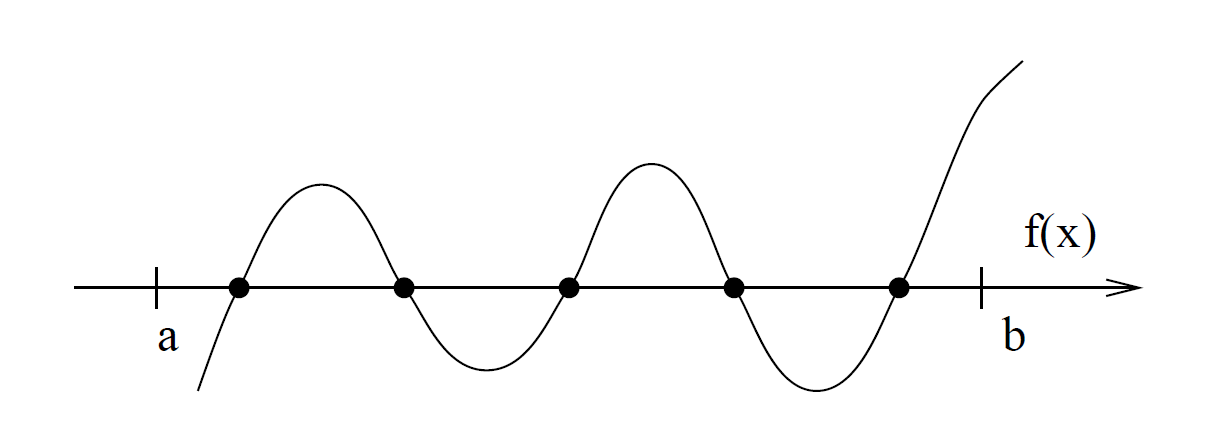
\includegraphics[width=1 \linewidth]{img/3/interpol_3_5}
	\end{figure}
Rysunek 3.2: Funkcja spełniająca założenia uogólnionego tw. Rolle'a 
 \end{frame}



 \begin{frame}

Założenia:

\begin{itemize}
\item $x_{0}, x_{1}$, . . . , $x_{n}\in[a,\ b]$ -- różne punkty
\item $P_{n}(x)$ -- wiel. interpolacyjny Lagrange'a
\item $f\in C^{(n+1)}[a,\ b]$
\end{itemize}

\begin{block}
{Teza:}
\begin{gather*}
  \forall x \in[a,\ b] \text{ } \exists \eta \in (a, b), \eta = \eta(x): \\ \\
  f(x)=P_{n}(x)+\frac{f^{n+1}(\eta)}{(n+1)!}\prod_{i=0}^{n}(x-x_{i})\ (\star)
\end{gather*}
\end{block}

\end{frame}

\begin{frame}
Dane:

$x=x_{k}, k=0$, 1, . . . , $n \rightarrow f(x_{k})=P_{n}(x_{k})\Rightarrow$dowolny $\eta$ spelnia $(\star)$ \newline
- dla ustalonego $x\neq x_{k}, k=0$, 1, . . . , $n\Rightarrow g(t)$ , $[a,\ b]$ :

$$g(t)=f(t)-P_{n}(t)-[f(x)-P_{n}(x)]\prod_{i=0}^{n}\frac{t-x_{i}}{x-x_{i}}$$

$$
 \left. \begin{array}{ll}
f\in C^{(n+1)}[a,\ b] \\
P\in C^{\infty}[a,\ b]\\
x\neq x_{k}
\end{array} \right \} \Rightarrow g(t)\in C^{(n+1)}[a,\ b]
$$

$\fbox{$t=x_{k}:$}$

$$g(x_{k})=\underbrace{f(x_{k})-P_{n}(x_{k})}_{=0}-[f(x)-P_{n}(x)]\underbrace{\prod_{i=0}^{n}\frac{x_{k}-x_{i}}{x-x_{i}}}_{=0}=0$$

\end{frame}

\begin{frame}
$\fbox{$t=x \neq x_k:$}$
$$
g(x)=f(x)-P_{n}(x)-[f(x)-P_{n}(x)]\underbrace{\prod_{i=0}^{n}\frac{x-x_{i}}{x-x_{i}}}_{=1}=0
$$
$\Rightarrow g(t)$ ma $(n+2)$ miejsc zerowych: $x, x_{0}, x_{1}$, . . . , $x_{n}$ \newline \newline
Zastosowanie twierdzenia Rolle'a:


$$\begin{array}{ll}
0=g^{(n+1)}(\displaystyle \eta)= \\
f^{(n+1)}(\eta)-\underbrace{P_{n}^{(n+1)}(\eta)}_{=0}-[f(x)-P_{n}(x)]\frac{d^{n+1}}{dx^{n+1}} \left \{\prod_{i=0}^{n}\frac{t-x_{i}}{x-x_{i}} \right \}_{t=\eta}  \end{array}$$


 \end{frame}

 \begin{frame}


$\displaystyle \prod_{i=0}^{n}\frac{t-x_{i}}{x-x_{i}}=\frac{t^{n+1}}{\prod_{i=0}^{n}(x-x_{i})}+at^{n}+\cdots$
$$
f^{(n+1)}(\eta)=[f(x)-P_{n}(x)]\frac{(n+1)!}{\prod_{i=0}^{n}(x-x_{i})}
$$
\textbf{Błąd interpolacji Lagrange'a:}
\begin{gather*}
  f(x)=P_{n}(x)+\underbrace{\frac{f^{(n+1)}(\eta)}{(n+1)!}\prod_{i=0}^{n}(x-x_{i})}_{\text{Porównaj z resztą Taylora!}}
\end{gather*}



\textbf{Zadanie:} Wyprowadź resztę Taylora powyższą metodą \\
\end{frame}

\begin{frame}
\begin{itemize}
\item Alternatywny zapis LIP: $(x_{0},\ x_{1},\ \ldots,\ x_{n})$ :
\end{itemize}
$\displaystyle \omega(x)=\prod_{k=0}^{n}(x-x_{k})$

$P_{n}(x)=\displaystyle \omega(x)\sum_{k=0}^{n}\frac{f(x_{k})}{(x-x_{k})\omega ^{'}(x_{k})}$ \\
\vspace{5mm}

\textbf{Zadanie:} Sprawdzić.

 \end{frame}
